\section{Suddivisione del lavoro}
I componenti del gruppo dovranno rivestire ognuno dei ruoli come specificato nella sezione
1.7.
\subsection{Analisi}
Nella fase di \textbf{Analisi} ciascun componente dovrà ricoprire i seguenti ruoli e per la quantità di ore specificate:

\begin{table}[H]
\centering
\begin{tabular}{|l|c|c|c|c|c|c|c|}
\hline
\textbf{Nominativo} & 
\multicolumn{6}{c|}{\textbf{Ore per ruolo}} & 
\textbf{Ore totali} \\
& Re & Am & An  & Pt & Ve & Pr & \\
\hline
Baggio Marco
  & 
  & 
  & 16
  & 
  & 6
  & 
  &
  22
  \\
Barcaro Andrea
  & 
  & 15.5
  & 3
  & 
  & 3
  & 
  &
 21.5
  \\
Garbin Simone
  & 10
  & 
  & 6
  & 
  & 6
  & 
  &
  22
  \\
Marchetto Pietro
  & 
  & 
  & 16
  & 
  & 6
  & 
  &
  22
  \\
Rodighiero Giovanni
  & 
  & 3
  & 6
  & 
  & 11
  & 
  &
  20
  \\
Speggiorin Federica
  & 16
  & 
  & 
  & 
  & 4
  & 
  &
  20
  \\
Todescato Filippo
  & 
  & 3
  & 16
  & 
  & 
  & 
  &
  19
  \\
\hline
\end{tabular}
\caption{Ore per componente, fase di Analisi}
\end{table}
I valori sopra riportati sono riassunti nel seguente grafico che mostra visivamente i ruoli assunti da ogni componente di \GroupName{} durante la fase di Analisi.
\begin{figure}[H]
\centering
\scalebox{0.6}{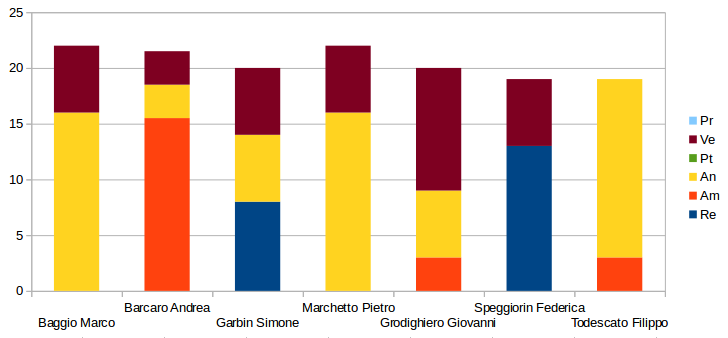
\includegraphics{img_ore/oreAnalisi.png}}
\caption{Ore per componente, fase di Analisi}
\end{figure}


\subsection{Incremento fase di Analisi}
\subsection{Progettazione Architetturale}
\subsection{Progettazione di dettaglio e codifica}
\subsection{Verifica e Validazione}
\subsection{Totale}





